%% ---------------------------------------------------------------------------------
\begin{frame}
  \titlepage
\end{frame}
%% ---------------------------------------------------------------------------------

%%%% ---------------------------------------------------------------------------------
\begin{frame}[c] \frametitle{Overview}
%  \framesubtitle{Untertitel}
  \begin{itemize} \setlength{\itemsep}{18pt}
    \item Introduction
    \item Problems with existing solutions
    \item Our solution
    \item Demo
  \end{itemize}
\end{frame}
%%%% ---------------------------------------------------------------------------------

\section{Introduction}
\sectionpage

%%%% ---------------------------------------------------------------------------------
%%%% Introduction
%%%% ---------------------------------------------------------------------------------
\begin{frame}[t]\frametitle{Introduction}
 \framesubtitle{What is remote signing?}
 \begin{columns}[T]
	\begin{column}{0.5\textwidth}
		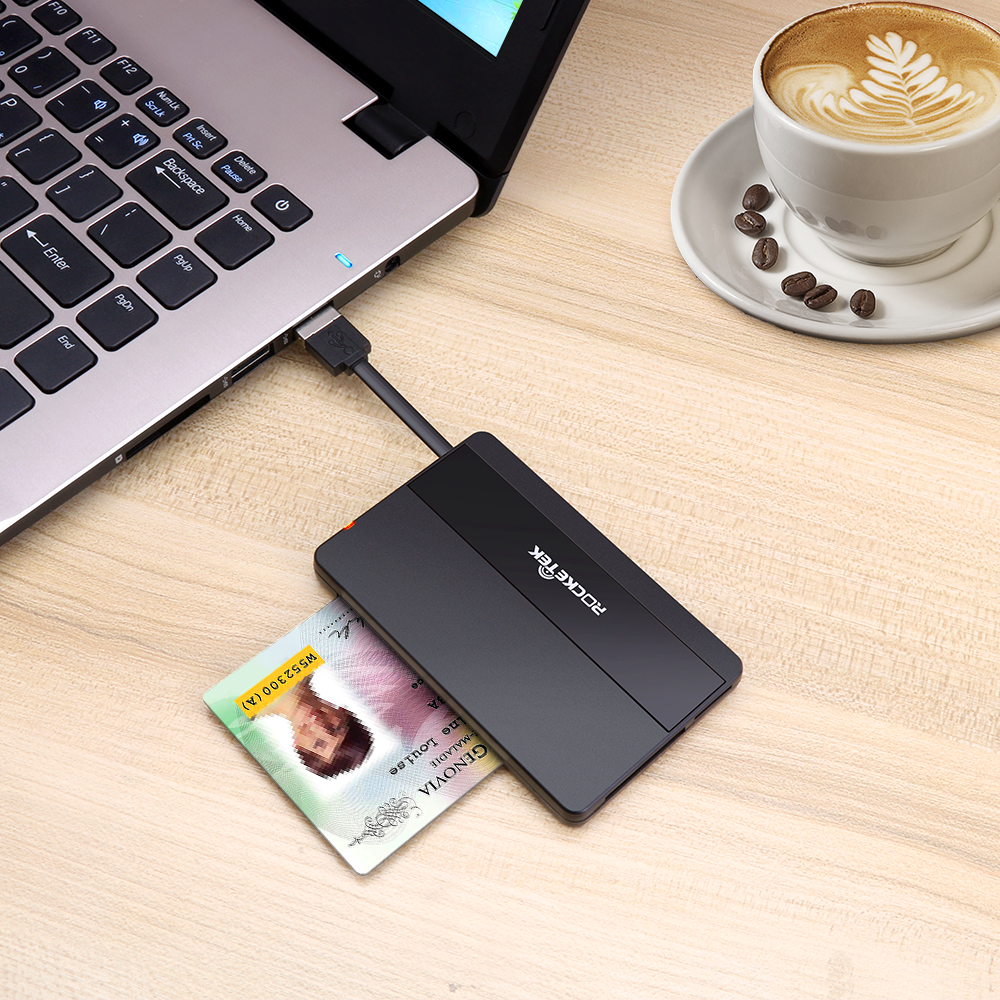
\includegraphics[width=\textwidth]{cardreader.jpg}
	\end{column}
	\begin{column}{0.5\textwidth}
		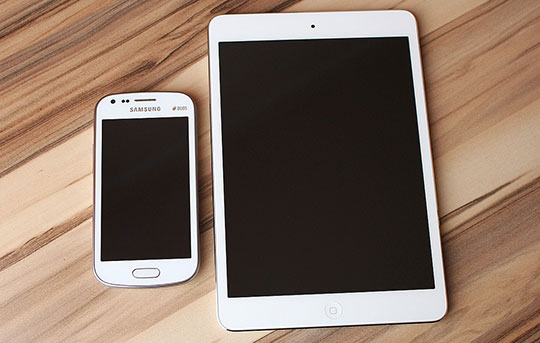
\includegraphics[width=\textwidth]{tablet-smartphone.jpg}
	\end{column}
 \end{columns}
\end{frame}

\begin{frame}[t]\frametitle{Introduction}
 \framesubtitle{What is remote signing?}
  \begin{itemize}
    \item Electronic signatures
    \begin{itemize}
      \item are legally binding
	  \item use digital signatures (cryptographic primitives)
    \end{itemize}
    \item No more hardware tokens
    \item Signing from every device, everywhere
    \item Signature Activation Protocol for unlocking the private key
  \end{itemize}
\end{frame}
%%%% ---------------------------------------------------------------------------------

\section{Problems with existing solutions}
\sectionpage


\begin{frame}[t]\frametitle{Problems with existing solutions}
	\framesubtitle{Adobe Sign}
	\begin{itemize}
	  \item Users don't have control of their private keys
      \item Signing Service can create signatures without the user's knowledge
      \item Trust-based Signature Activation Protocol
      \item Has access to your documents
	  \item Implementation is absolutely proprietary
	  \item Only possible to sign PDFs
	\end{itemize}
\end{frame}


\section{Our Solution}
\sectionpage

\begin{frame}[t]\frametitle{Our Solution}
	\framesubtitle{Big Picture}
	\begin{figure}[ht]
		\centering
		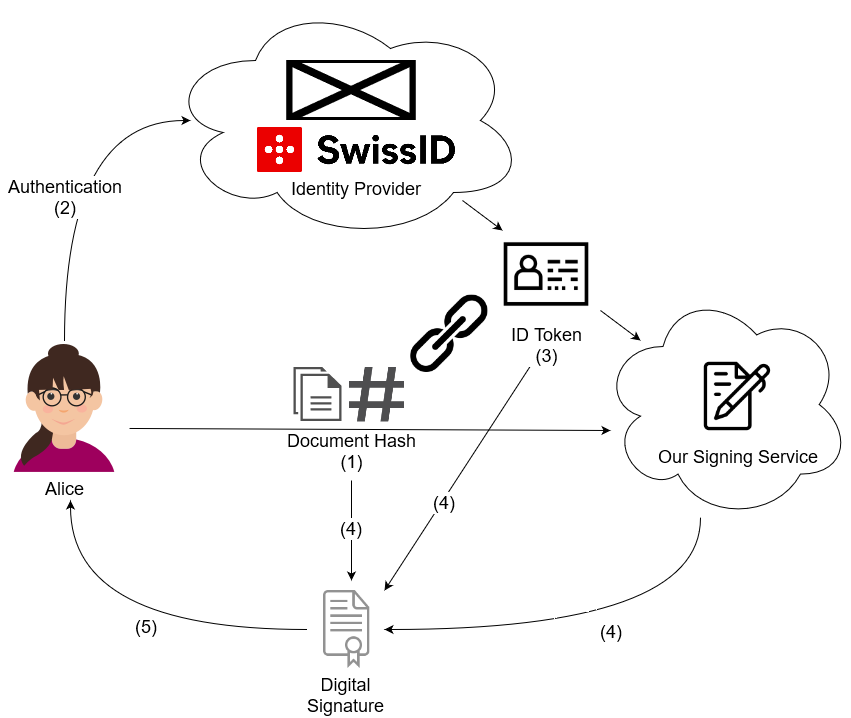
\includegraphics[scale=0.22]{BigPicture_v4.png}
	\end{figure}
\end{frame}

\begin{frame}[t]\frametitle{Our Solution}
	\framesubtitle{Overview}
	\begin{itemize}
		\item Trust is distributed between IdP and Signing Service
		\item Sign arbitrary documents
		\item Signing Service only receives hash of document
		\item Runs in the browser (no additional software necessary)
		\item Verifyable Signature Activation Protocol
		\item Offline verification
		\item Uses standard technologies (OIDC, CMS, X.509)
	\end{itemize}
\end{frame}

\begin{frame}[t]{Our Solution}
	\framesubtitle{Protocol Overview}
	\begin{figure}[ht]
		\centering
		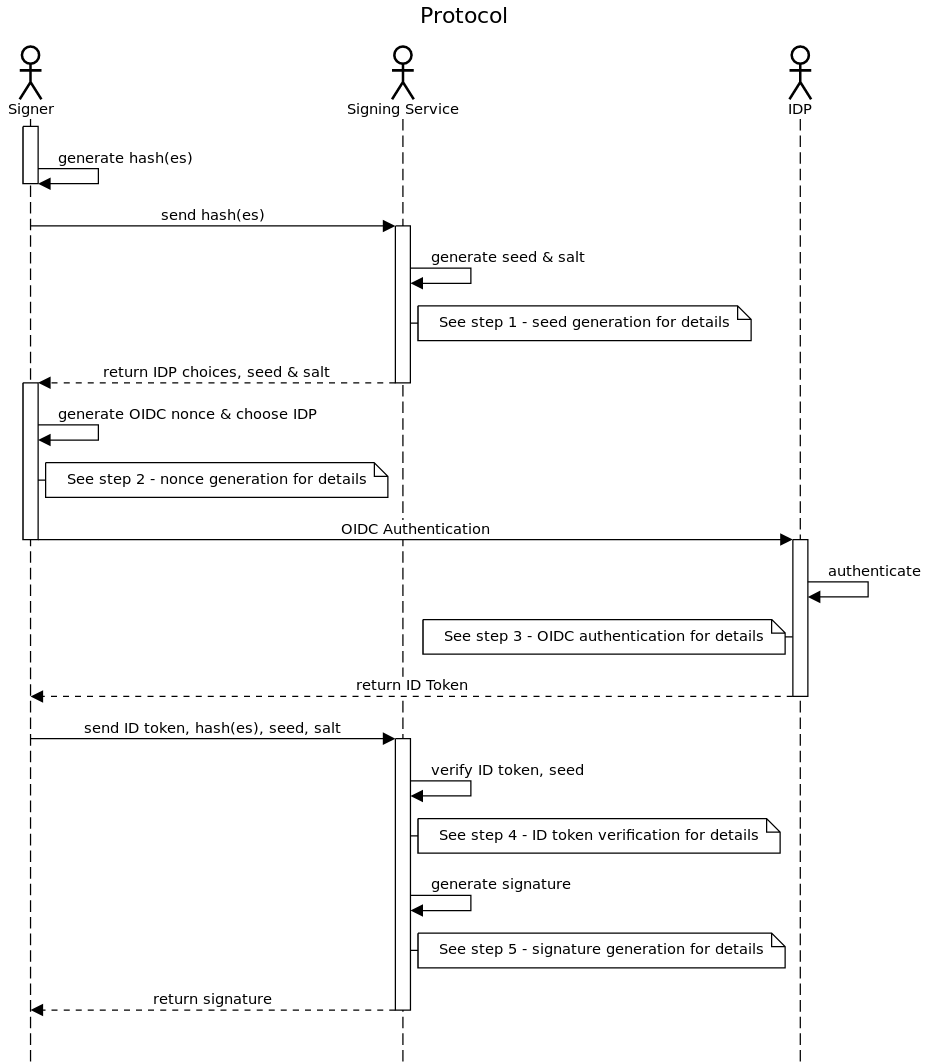
\includegraphics[scale=0.18]{protocol_signature_generation_high_level.png}
	\end{figure}
\end{frame}

\begin{frame}[t]{Our Solution}
	\framesubtitle{Step 1 - Seed generation}
	\begin{figure}[ht]
		\centering
		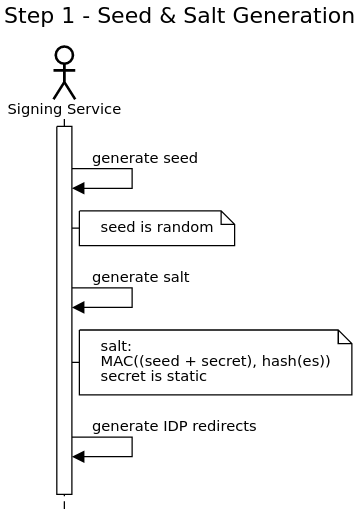
\includegraphics[scale=0.13]{protocol_step1_seed_generation.png}
	\end{figure}
\end{frame}

\begin{frame}[t]{Our Solution}
	\framesubtitle{Step 2 - Nonce generation}
	\begin{figure}[ht]
		\centering
		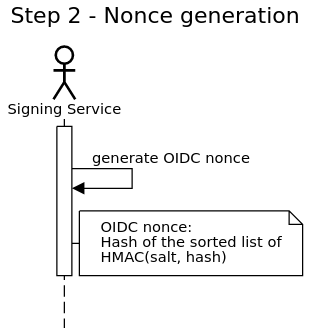
\includegraphics[scale=0.13]{protocol_step2_nonce_generation.png}
	\end{figure}
\end{frame}

\begin{frame}[t]{Our Solution}
	\framesubtitle{Step 3 - OIDC Authentication}
	\begin{figure}[ht]
		\centering
		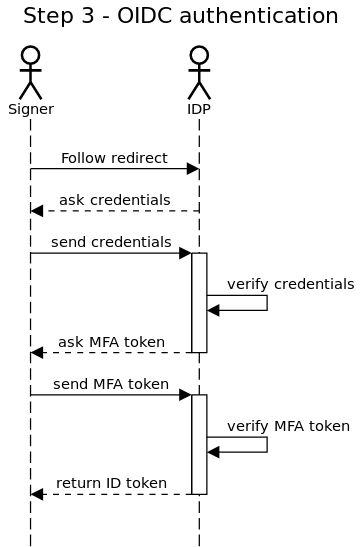
\includegraphics[scale=0.1]{protocol_step3_oidc_authentication.png}
	\end{figure}
\end{frame}

\begin{frame}[t]{Our Solution}
	\framesubtitle{Step 4 - ID token verification}
	\begin{figure}[ht]
		\centering
		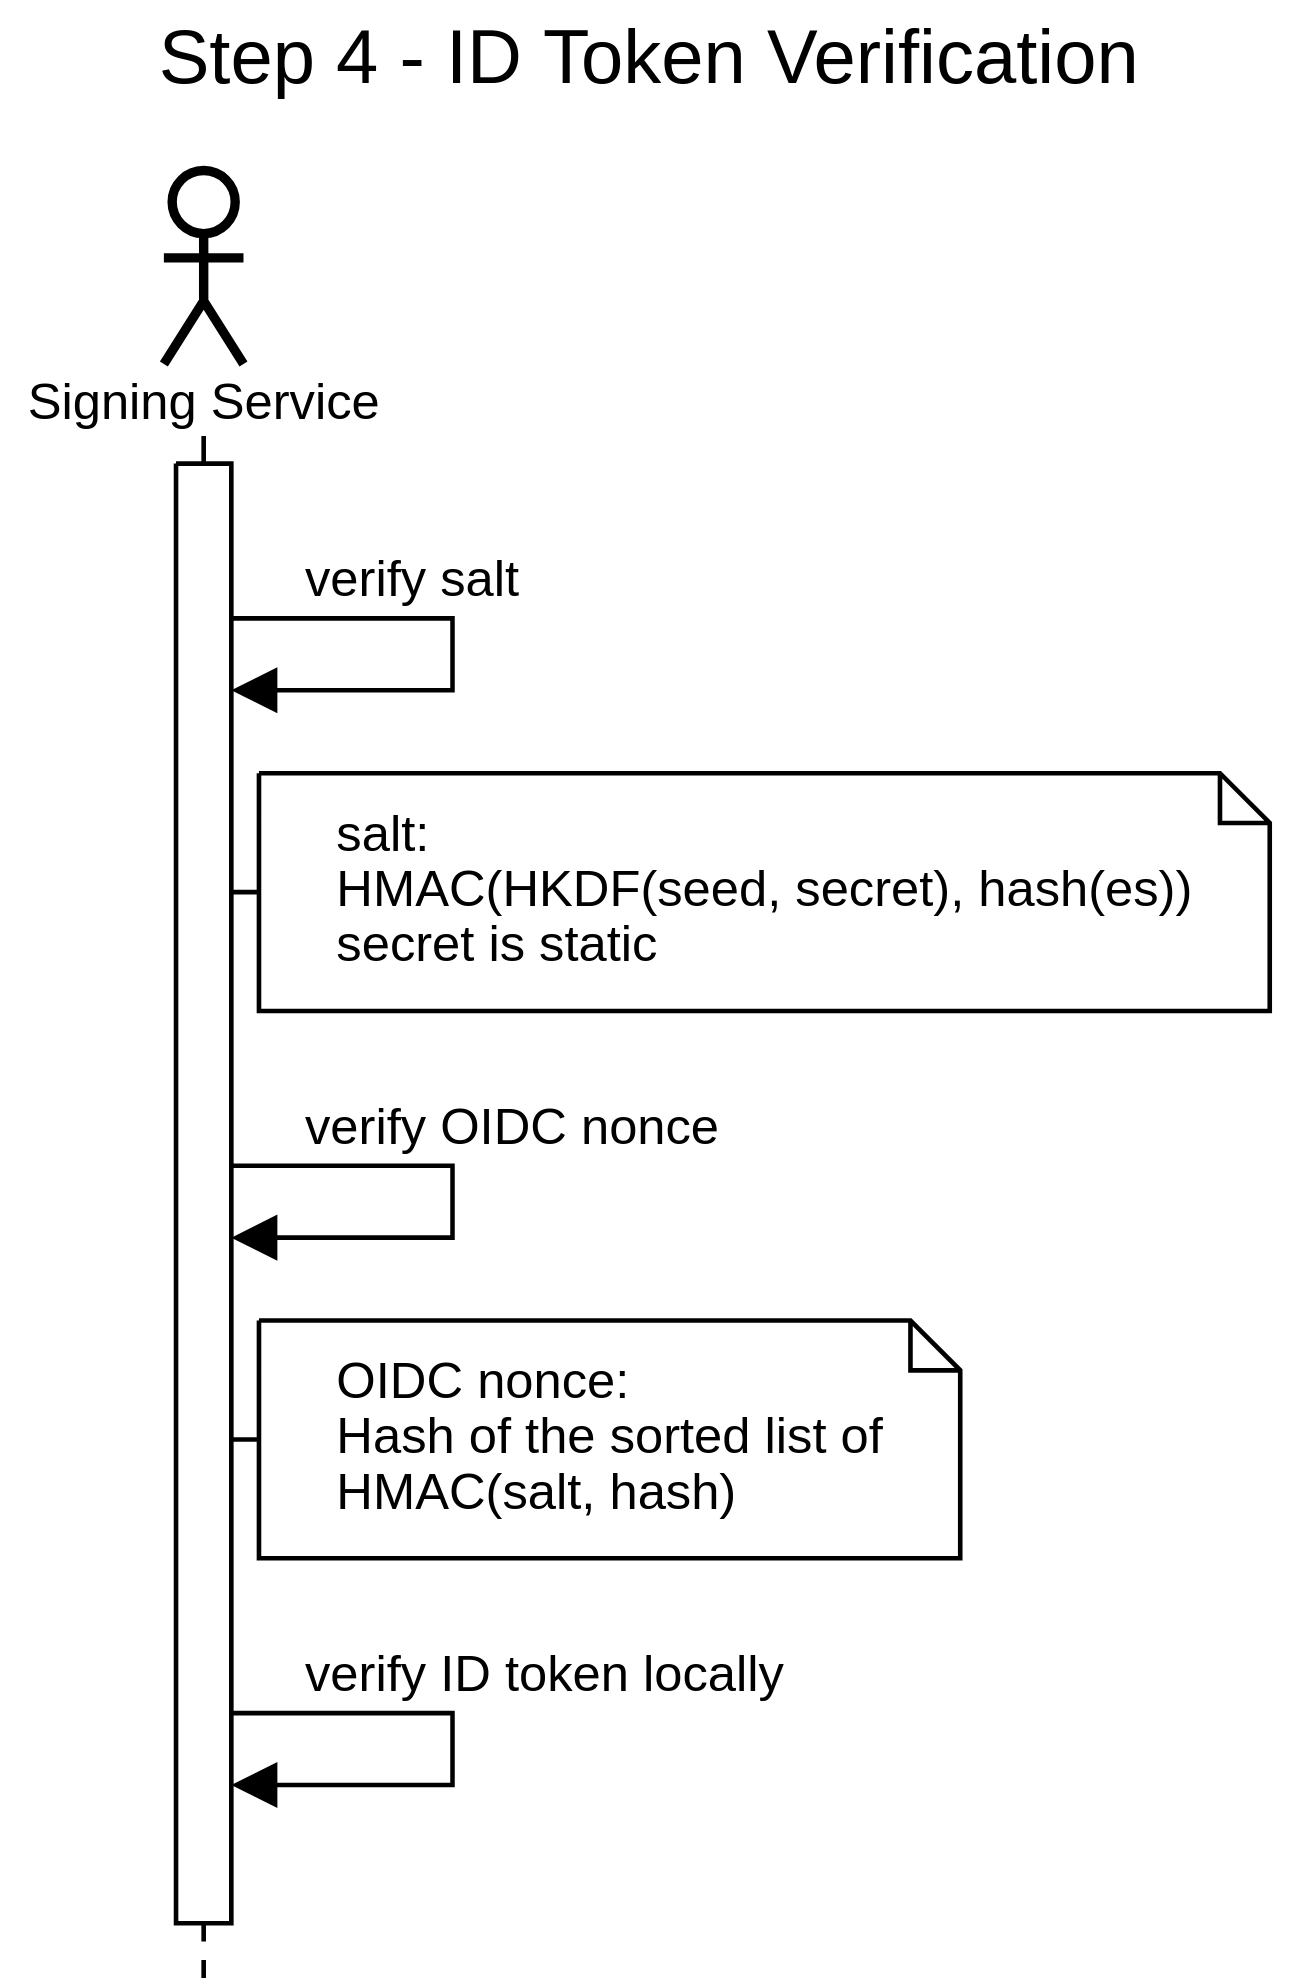
\includegraphics[scale=0.1]{protocol_step4_id_token_verification.png}
	\end{figure}
\end{frame}

\begin{frame}[t]{Our Solution}
	\framesubtitle{Step 5 - Signature Generation}
	\begin{figure}[ht]
		\centering
		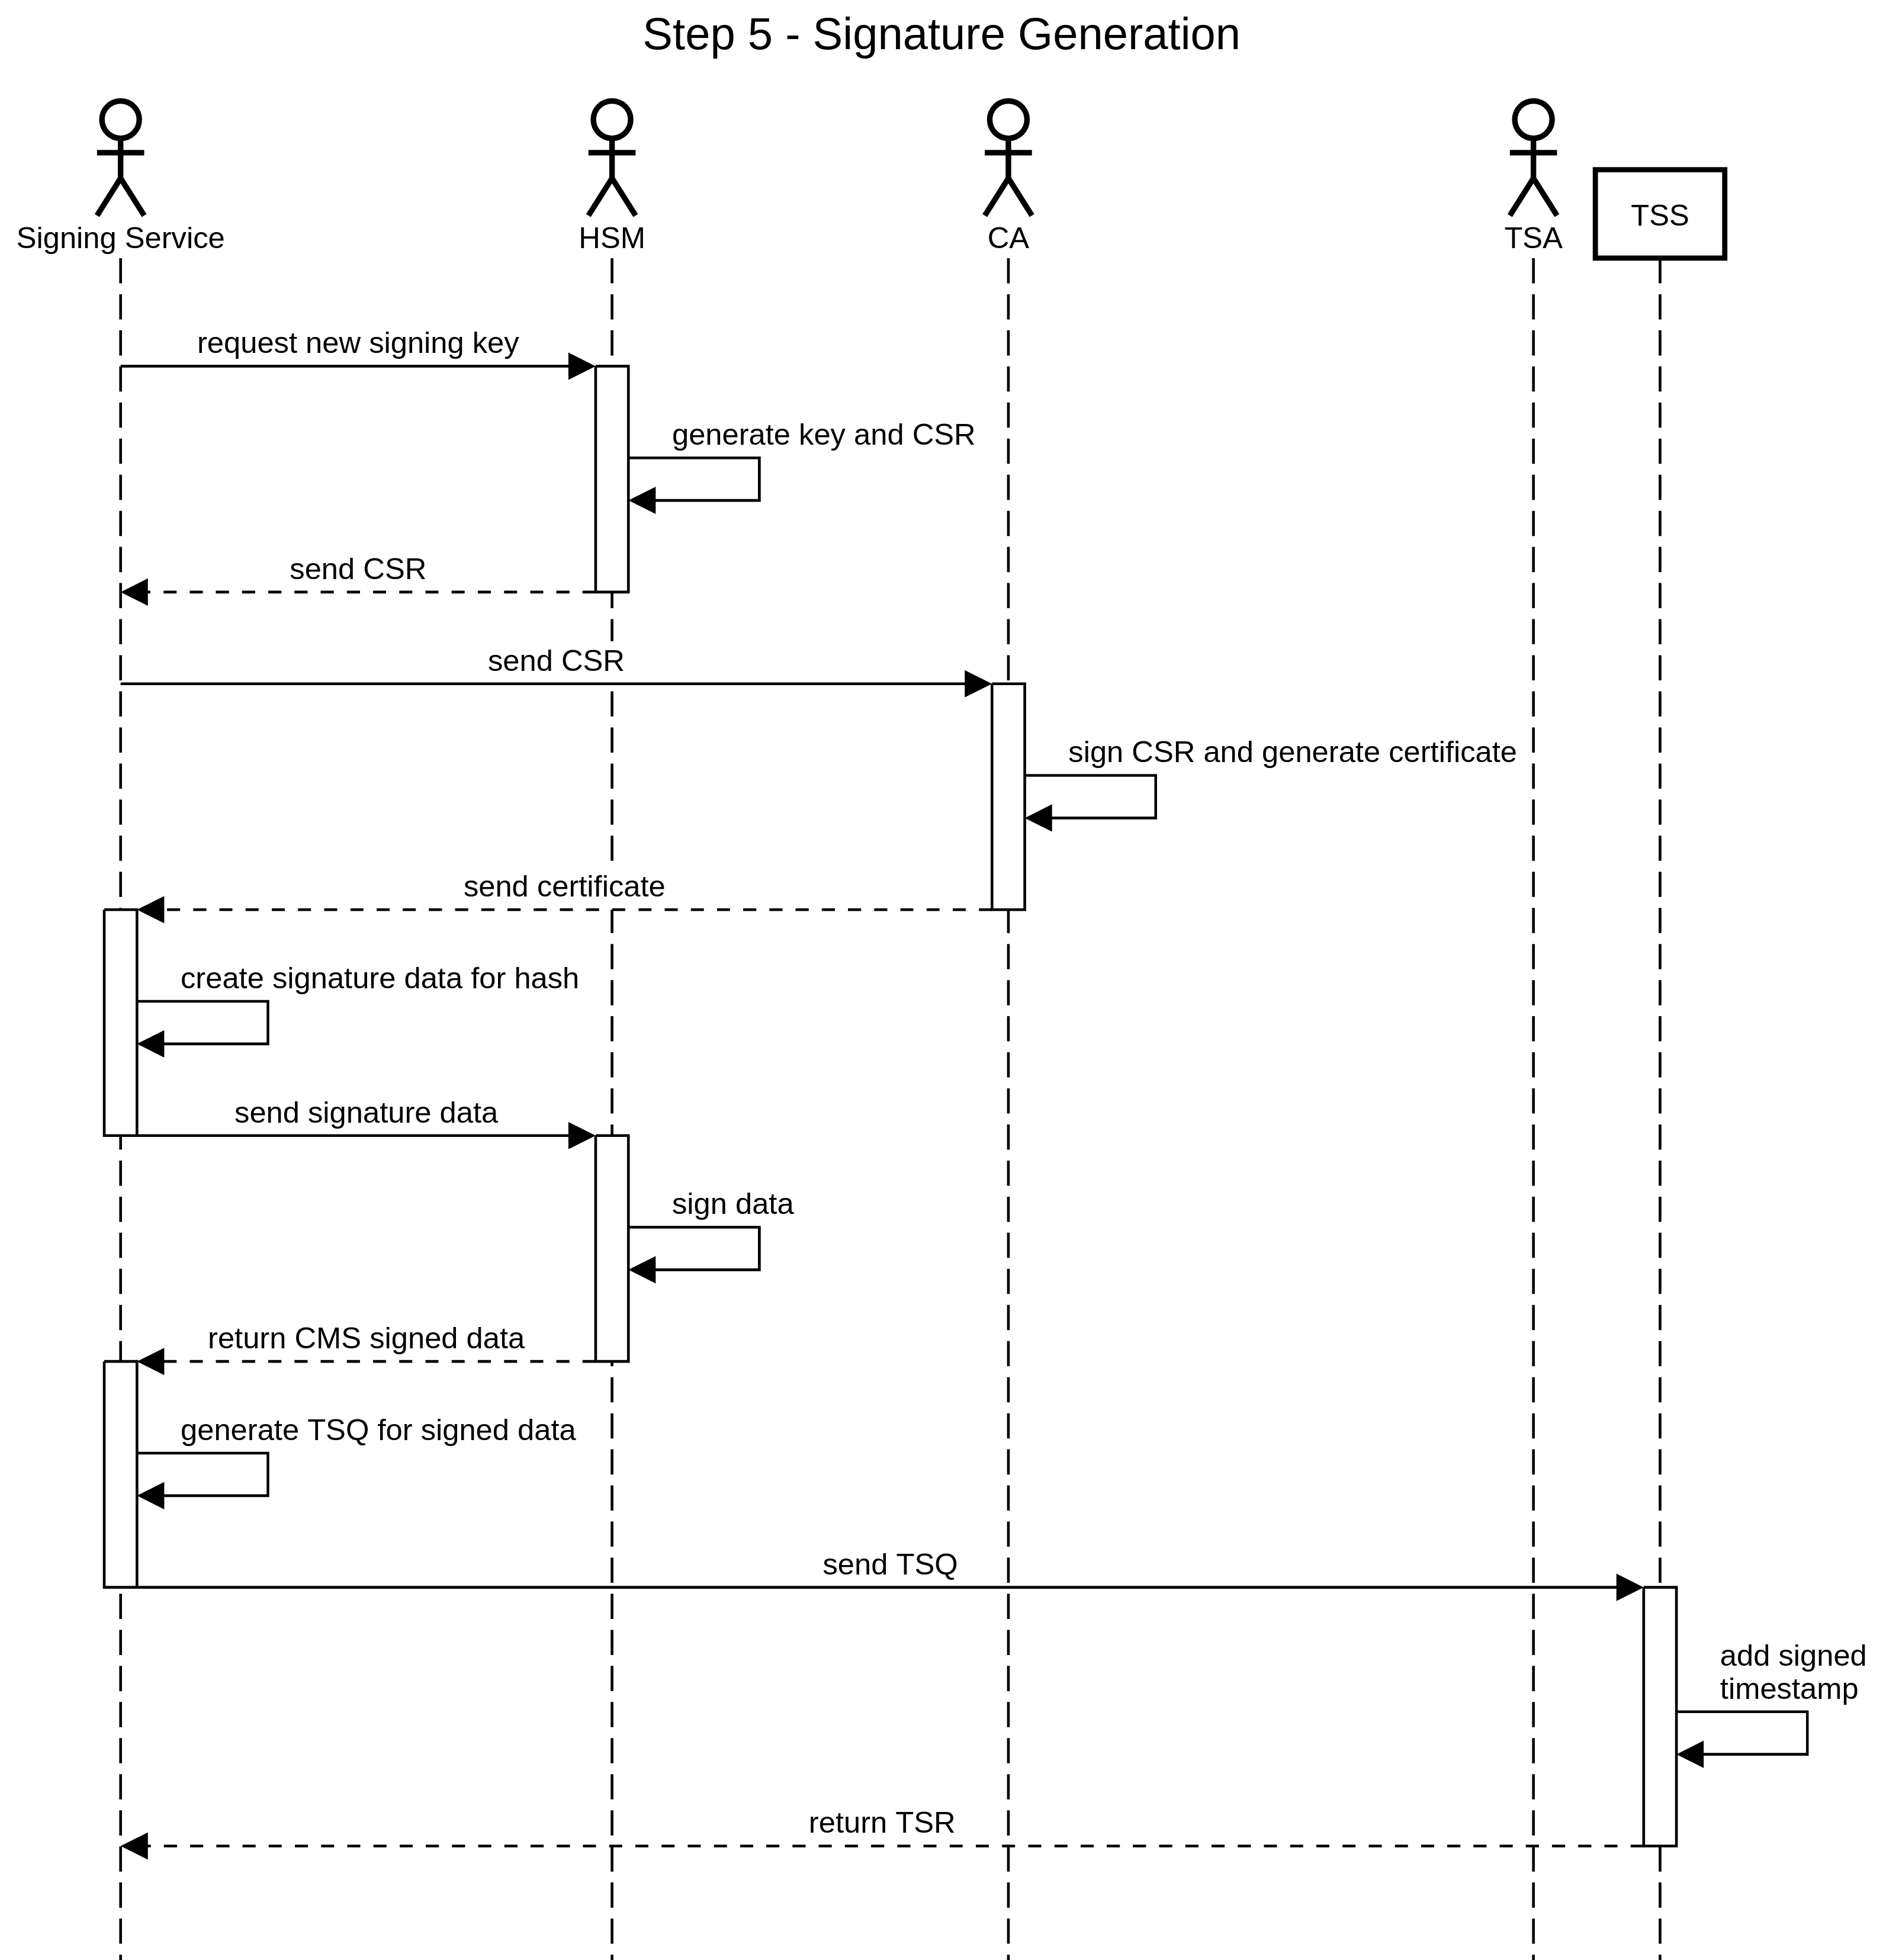
\includegraphics[scale=0.06]{protocol_step5_signature_generation.png}
	\end{figure}
\end{frame}

\begin{frame}[t]\frametitle{Our Solution}
	\framesubtitle{How we do it}
	\begin{itemize}
		\item Reuse the nonce in the OIDC ID token
		\begin{itemize}
			\item nonce consists of list of salted hashes of the documents
			\item couples documents with the ID token
		\end{itemize}
		\item Signing Service can only sign the hashes which flow into the nonce
		\item Signature is detached
		\item All certificate chains and revocation info (CRL/OCSP) are in the signature for offline verification
	\end{itemize}
\end{frame}

\begin{frame}[t]\frametitle{Our Solution}
	\framesubtitle{Signature Format}
	\begin{figure}[ht]
		\centering
		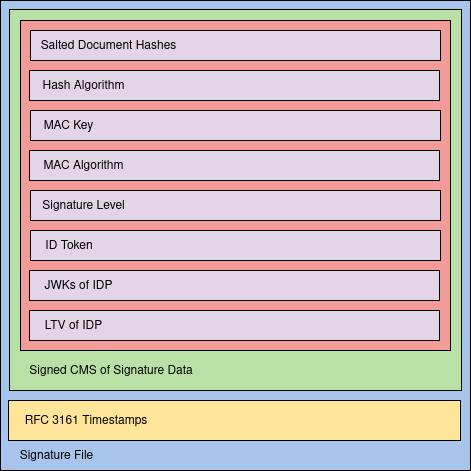
\includegraphics[scale=0.4]{signature_file.png}
	\end{figure}
\end{frame}

\section{Demo}
\sectionpage

\section{Questions?}
\sectionpage
